\documentclass{standalone}
\usepackage{tikz}
\usetikzlibrary{patterns, positioning}
\usepackage[sfdefault]{ClearSans} %% option 'sfdefault' activates Clear Sans as the default text font
\usepackage[T1]{fontenc}

\begin{document}
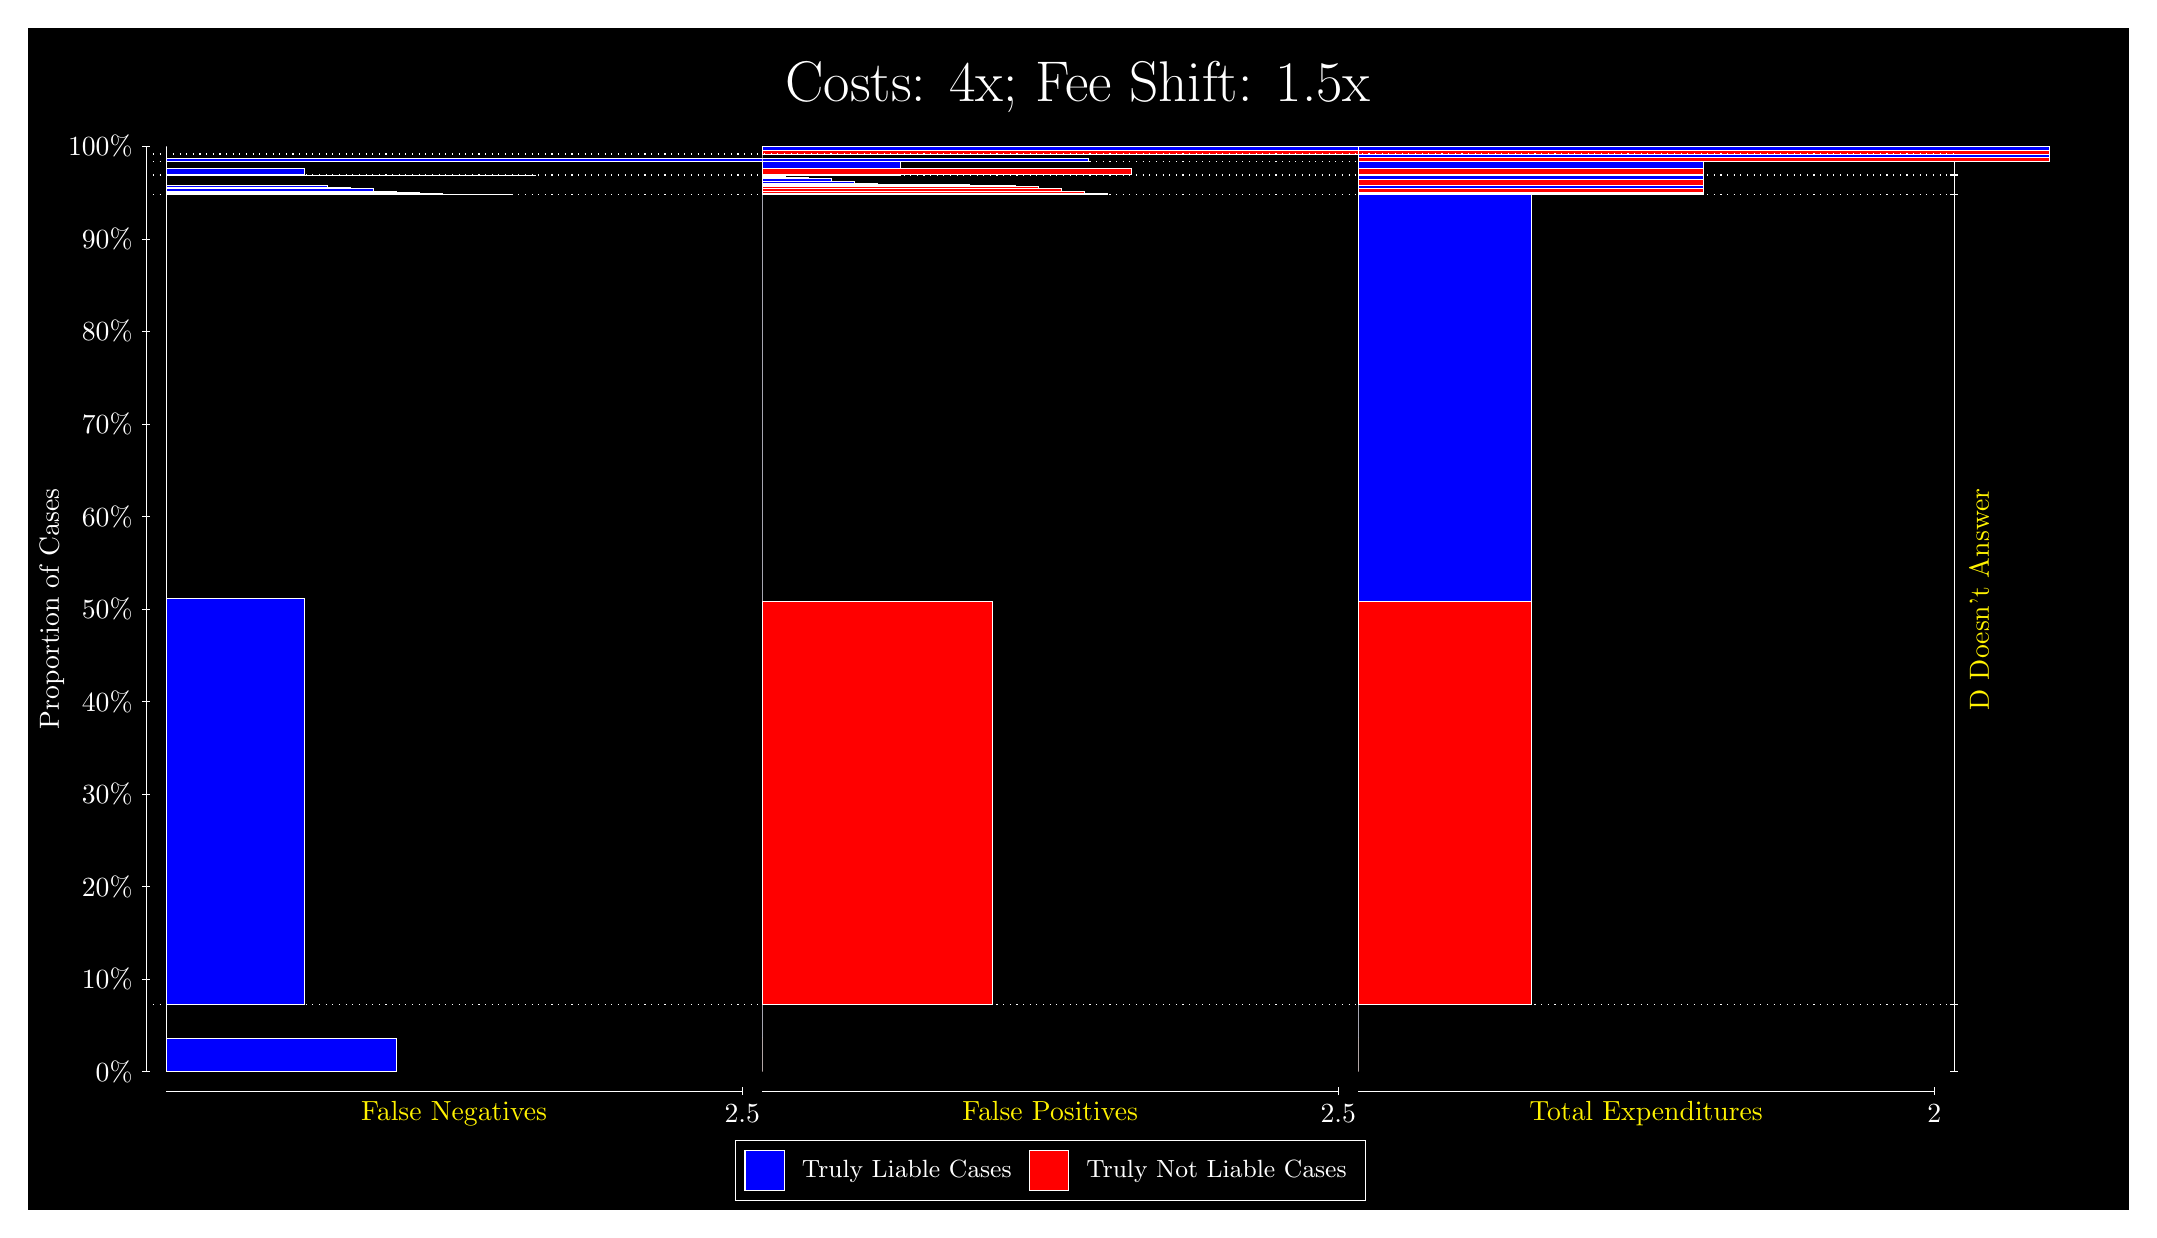
\begin{tikzpicture}
\draw[fill=black] (0,0) rectangle (26.667,15);
\draw[text=white] (0,13.5) rectangle (26.667,15) node[midway] {\huge Costs: 4x; Fee Shift: 1.5x};
\draw[white, very thin] (1.5,1.75) -- (1.5,13.5);
\node[rotate=90, text=white, anchor=center] at (0.3, 7.625) {Proportion of Cases};
\draw[white, very thin] (1.45,1.75) -- (1.55,1.75);
\node[text=white, anchor=east] at (1.45, 1.75) {0\%};
\draw[white, very thin] (1.45,2.925) -- (1.55,2.925);
\node[text=white, anchor=east] at (1.45, 2.925) {10\%};
\draw[white, very thin] (1.45,4.1) -- (1.55,4.1);
\node[text=white, anchor=east] at (1.45, 4.1) {20\%};
\draw[white, very thin] (1.45,5.275) -- (1.55,5.275);
\node[text=white, anchor=east] at (1.45, 5.275) {30\%};
\draw[white, very thin] (1.45,6.45) -- (1.55,6.45);
\node[text=white, anchor=east] at (1.45, 6.45) {40\%};
\draw[white, very thin] (1.45,7.625) -- (1.55,7.625);
\node[text=white, anchor=east] at (1.45, 7.625) {50\%};
\draw[white, very thin] (1.45,8.8) -- (1.55,8.8);
\node[text=white, anchor=east] at (1.45, 8.8) {60\%};
\draw[white, very thin] (1.45,9.975) -- (1.55,9.975);
\node[text=white, anchor=east] at (1.45, 9.975) {70\%};
\draw[white, very thin] (1.45,11.15) -- (1.55,11.15);
\node[text=white, anchor=east] at (1.45, 11.15) {80\%};
\draw[white, very thin] (1.45,12.325) -- (1.55,12.325);
\node[text=white, anchor=east] at (1.45, 12.325) {90\%};
\draw[white, very thin] (1.45,13.5) -- (1.55,13.5);
\node[text=white, anchor=east] at (1.45, 13.5) {100\%};

\draw[white, very thin] (24.457,1.75) -- (24.457,13.5);
\draw[white, very thin] (24.407,1.75) -- (24.507,1.75);
\node[anchor=west] at (24.407, 1.75) {};
\draw[white, very thin] (24.407,2.602) -- (24.507,2.602);
\node[anchor=west] at (24.407, 2.602) {};
\draw[white, very thin] (24.407,12.888) -- (24.507,12.888);
\node[anchor=west] at (24.407, 12.888) {};
\draw[white, very thin] (24.407,13.13) -- (24.507,13.13);
\node[anchor=west] at (24.407, 13.13) {};
\draw[white, very thin] (24.407,13.14) -- (24.507,13.14);
\node[anchor=west] at (24.407, 13.14) {};
\draw[white, very thin] (24.407,13.304) -- (24.507,13.304);
\node[anchor=west] at (24.407, 13.304) {};
\draw[white, very thin] (24.407,13.403) -- (24.507,13.403);
\node[anchor=west] at (24.407, 13.403) {};
\draw[white, very thin] (24.407,13.5) -- (24.507,13.5);
\node[anchor=west] at (24.407, 13.5) {};

\draw[white, very thin, fill=blue] (1.75,1.75) rectangle (4.6775,2.176);
\draw[white, very thin, fill=red] (1.75,2.176) rectangle (1.75,2.602);
\draw[white, very thin, fill=blue] (1.75,2.602) rectangle (3.5065,7.7655);
\draw[white, very thin, fill=red] (1.75,7.7655) rectangle (1.75,12.888);
\draw[white, very thin, fill=blue] (1.75,12.888) rectangle (6.1413,12.89);
\draw[white, very thin, fill=blue] (1.75,12.89) rectangle (5.8486,12.892);
\draw[white, very thin, fill=blue] (1.75,12.892) rectangle (5.5558,12.895);
\draw[white, very thin, fill=blue] (1.75,12.895) rectangle (5.2631,12.899);
\draw[white, very thin, fill=blue] (1.75,12.899) rectangle (4.9703,12.914);
\draw[white, very thin, fill=blue] (1.75,12.914) rectangle (4.6775,12.928);
\draw[white, very thin, fill=blue] (1.75,12.928) rectangle (4.3848,12.961);
\draw[white, very thin, fill=blue] (1.75,12.961) rectangle (4.092,12.982);
\draw[white, very thin, fill=blue] (1.75,12.982) rectangle (3.7993,13);
\draw[white, very thin, fill=red] (1.75,13) rectangle (1.75,13.13);
\draw[white, very thin, fill=blue] (1.75,13.13) rectangle (6.4341,13.135);
\draw[white, very thin, fill=red] (1.75,13.135) rectangle (1.75,13.14);
\draw[white, very thin, fill=blue] (1.75,13.14) rectangle (3.5065,13.217);
\draw[white, very thin, fill=red] (1.75,13.217) rectangle (1.75,13.304);
\draw[white, very thin, fill=blue] (1.75,13.304) rectangle (13.46,13.347);
\draw[white, very thin, fill=red] (1.75,13.347) rectangle (1.75,13.403);
\draw[white, very thin, fill=red] (1.75,13.403) rectangle (1.75,13.451);
\draw[white, very thin, fill=blue] (1.75,13.451) rectangle (1.75,13.5);
\draw[white, very thin, fill=red] (9.3189,1.75) rectangle (9.3189,2.176);
\draw[white, very thin, fill=blue] (9.3189,2.176) rectangle (9.3189,2.602);
\draw[white, very thin, fill=red] (9.3189,2.602) rectangle (12.246,7.7245);
\draw[white, very thin, fill=blue] (9.3189,7.7245) rectangle (9.3189,12.888);
\draw[white, very thin, fill=red] (9.3189,12.888) rectangle (13.71,12.907);
\draw[white, very thin, fill=red] (9.3189,12.907) rectangle (13.417,12.932);
\draw[white, very thin, fill=red] (9.3189,12.932) rectangle (13.125,12.972);
\draw[white, very thin, fill=red] (9.3189,12.972) rectangle (12.832,12.988);
\draw[white, very thin, fill=red] (9.3189,12.988) rectangle (12.539,13.006);
\draw[white, very thin, fill=red] (9.3189,13.006) rectangle (12.246,13.01);
\draw[white, very thin, fill=red] (9.3189,13.01) rectangle (11.954,13.014);
\draw[white, very thin, fill=red] (9.3189,13.014) rectangle (11.661,13.017);
\draw[white, very thin, fill=red] (9.3189,13.017) rectangle (11.368,13.018);
\draw[white, very thin, fill=blue] (9.3189,13.018) rectangle (10.783,13.036);
\draw[white, very thin, fill=blue] (9.3189,13.036) rectangle (10.49,13.057);
\draw[white, very thin, fill=blue] (9.3189,13.057) rectangle (10.197,13.091);
\draw[white, very thin, fill=blue] (9.3189,13.091) rectangle (9.9044,13.104);
\draw[white, very thin, fill=blue] (9.3189,13.104) rectangle (9.6116,13.12);
\draw[white, very thin, fill=blue] (9.3189,13.12) rectangle (9.3189,13.13);
\draw[white, very thin, fill=red] (9.3189,13.13) rectangle (11.075,13.135);
\draw[white, very thin, fill=blue] (9.3189,13.135) rectangle (9.3189,13.14);
\draw[white, very thin, fill=red] (9.3189,13.14) rectangle (14.003,13.227);
\draw[white, very thin, fill=blue] (9.3189,13.227) rectangle (11.075,13.304);
\draw[white, very thin, fill=red] (9.3189,13.304) rectangle (9.3189,13.361);
\draw[white, very thin, fill=blue] (9.3189,13.361) rectangle (9.3189,13.403);
\draw[white, very thin, fill=red] (9.3189,13.403) rectangle (21.029,13.451);
\draw[white, very thin, fill=blue] (9.3189,13.451) rectangle (18.102,13.5);
\draw[white, very thin, fill=red] (16.888,1.75) rectangle (16.888,2.176);
\draw[white, very thin, fill=blue] (16.888,2.176) rectangle (16.888,2.602);
\draw[white, very thin, fill=red] (16.888,2.602) rectangle (19.083,7.7245);
\draw[white, very thin, fill=blue] (16.888,7.7245) rectangle (19.083,12.888);
\draw[white, very thin, fill=red] (16.888,12.888) rectangle (21.279,12.906);
\draw[white, very thin, fill=blue] (16.888,12.906) rectangle (21.279,12.922);
\draw[white, very thin, fill=red] (16.888,12.922) rectangle (21.279,12.969);
\draw[white, very thin, fill=blue] (16.888,12.969) rectangle (21.279,13.011);
\draw[white, very thin, fill=red] (16.888,13.011) rectangle (21.279,13.076);
\draw[white, very thin, fill=blue] (16.888,13.076) rectangle (21.279,13.13);
\draw[white, very thin, fill=red] (16.888,13.13) rectangle (21.279,13.135);
\draw[white, very thin, fill=blue] (16.888,13.135) rectangle (21.279,13.14);
\draw[white, very thin, fill=red] (16.888,13.14) rectangle (21.279,13.227);
\draw[white, very thin, fill=blue] (16.888,13.227) rectangle (21.279,13.304);
\draw[white, very thin, fill=red] (16.888,13.304) rectangle (25.67,13.361);
\draw[white, very thin, fill=blue] (16.888,13.361) rectangle (25.67,13.403);
\draw[white, very thin, fill=red] (16.888,13.403) rectangle (25.67,13.451);
\draw[white, very thin, fill=blue] (16.888,13.451) rectangle (25.67,13.5);
\draw[white, dotted] (1.5,2.602) -- (24.457,2.602);
\draw[white, dotted] (1.5,12.888) -- (24.457,12.888);
\draw[white, dotted] (1.5,13.13) -- (24.457,13.13);
\draw[white, dotted] (1.5,13.14) -- (24.457,13.14);
\draw[white, dotted] (1.5,13.304) -- (24.457,13.304);
\draw[white, dotted] (1.5,13.403) -- (24.457,13.403);
\draw[white, very thin] (1.75,1.5) -- (9.0689,1.5);
\node[text=yellow, anchor=north] at (5.4094, 1.5) {False Negatives};
\draw[white, very thin] (9.0689,1.45) -- (9.0689,1.55);
\node[text=white, anchor=north] at (9.0689, 1.45) {2.5};

\draw[white, very thin] (9.3189,1.5) -- (16.638,1.5);
\node[text=yellow, anchor=north] at (12.978, 1.5) {False Positives};
\draw[white, very thin] (16.638,1.45) -- (16.638,1.55);
\node[text=white, anchor=north] at (16.638, 1.45) {2.5};

\draw[white, very thin] (16.888,1.5) -- (24.207,1.5);
\node[text=yellow, anchor=north] at (20.547, 1.5) {Total Expenditures};
\draw[white, very thin] (24.207,1.45) -- (24.207,1.55);
\node[text=white, anchor=north] at (24.207, 1.45) {2};


\node[text=yellow, centered, rotate=90] at (24.777, 7.745) {D Doesn't Answer};






\draw (12.978300999999998,1.5) node[draw=none] (baseCoordinate) {};
\begin{scope}[align=center]
        \matrix[scale=0.5, draw=white, below=0.5cm of baseCoordinate, nodes={draw}, column sep=0.1cm]{
            \node[rectangle, draw, minimum width=0.5cm, minimum height=0.5cm, fill=blue] {}; &
            \node[draw=none, font=\small, text=white] (B) {Truly Liable Cases}; &
            \node[rectangle, draw, minimum width=0.5cm, minimum height=0.5cm, fill=red] {}; &
            \node[draw=none, font=\small, text=white] (B) {Truly Not Liable Cases}; \\
            };
\end{scope}

\end{tikzpicture}
\end{document}